\subsubsection{Pix2Pix}

\subsubsubsection{Redes Generativas Antagónicas}

Las Redes Generativas Antagónicas (GAN's) es un modelo que se enfrenta contra un modelo discriminativo que aprende a determinar cuando una muestra es producida por un modelo o es de los datos.

\subsubsubsection{Estructura de modelación}

Los problemas de imagen a imagen por lo regular son tratados como una clasificación pixel a pixel. Para ello, cada pixel es tratado con una probabilidad independiente a su alrededor. Las GANs condicionales aprenden una estructura de perdida, la cual penaliza las diferencias entre la configuración final y la configuración objetivo.

\subsubsubsection{Arquitectura}

Para definir el problema de la traducción imagen a imagen, es definir una imagen de alta resolución que difiere en apariencia a la imagen de salida. Es por ello que la estructura en la entrada difiere a la de salida. Es por ello que se considero un generador que considera estas propiedades. Las soluciones propuestas con anterioridad es el uso de una red encoder-decoder.  En estas redes la información atraviesa una serie de capas que reducen su dimensión hasta llegar a una capa del tipo bottleneck, en seguida la información pasa por un proceso de expansión. Para muchos problemas de traducción de imagen es una gran idea realizar una conexión entre la entrada y la salida. Para implementar esta idea se añaden conexiones formando una red de tipo U-Net. Especificamente se añaden conexiones entre la capa $i$ y la capa $n-i$. En la figura \ref{fig:pix2pix} se visualiza la arquitectura de pix2pix.

\begin{figure}[H]
    \centering
    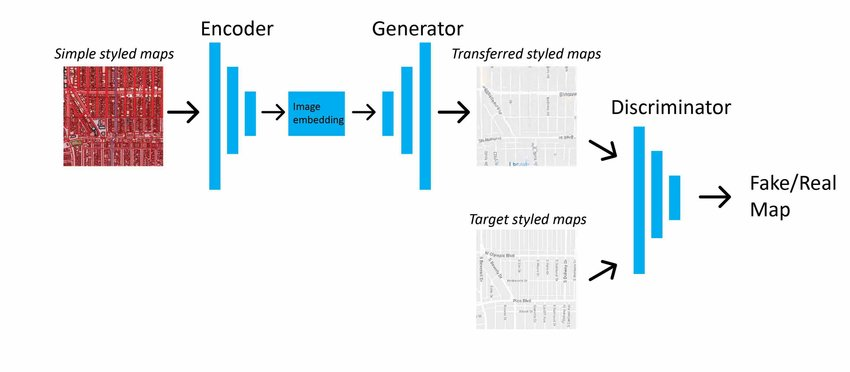
\includegraphics[width=16cm]{Graphics/pix2pix.jpg}
    \caption{Arquitectura de pix2pix\cite{Salimans_2016}.}
    \label{fig:pix2pix}
\end{figure}